
\begin{frame}{Cheating}
        \begin{exampleblock}{Question}
            How does a cheater determine which value to give his ratings in order to maximize (or minimize) a final rating? He can't!
        \end{exampleblock}
        
        \begin{figure}
            \centering
            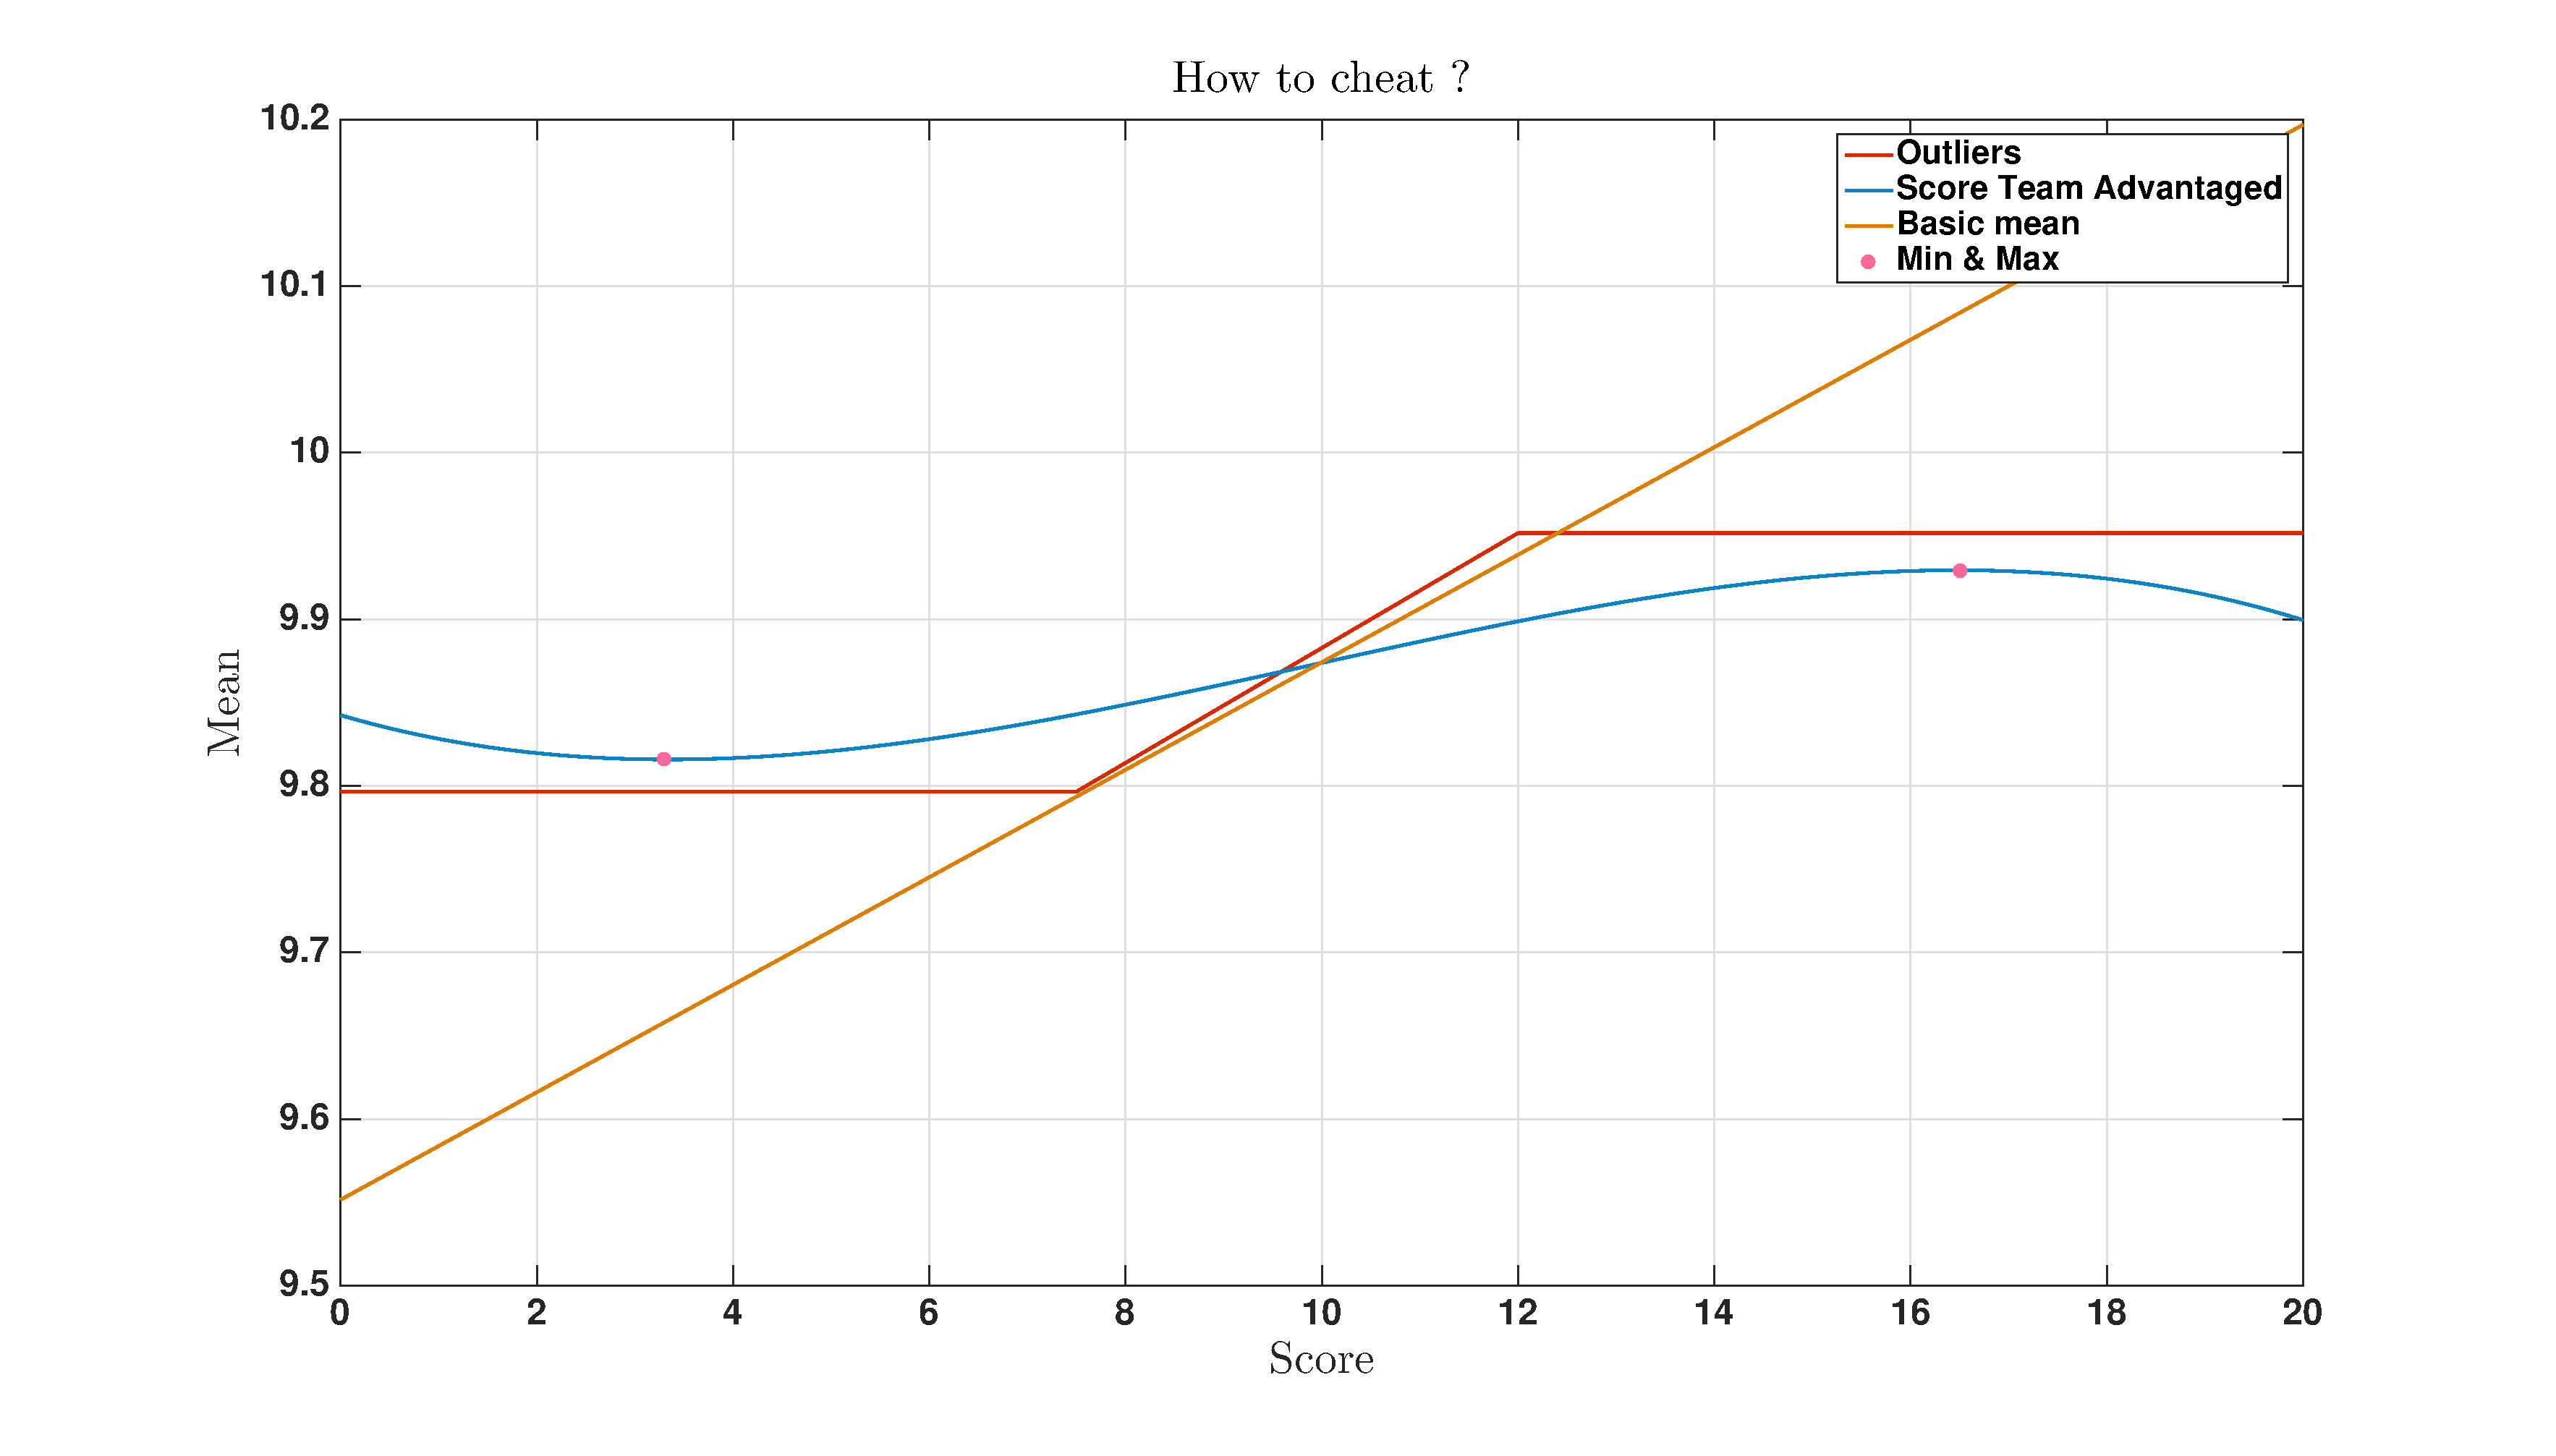
\includegraphics[width=\textwidth]{../rapport/images/cheaters/howto.eps}
        \end{figure}
\end{frame}

\begin{frame}{Application \rom{1}: MAP Scores}

\end{frame}

\usebackgroundtemplate{%
    \tikz\node[opacity=0.1] {
\includegraphics[height=\paperheight]{images/tripadvisor.jpg}};
}
\begin{frame}{Application \rom{2}: Hotels}
\begin{itemize}
    \item Subset of \textit{TripAdvisor}:
    \begin{itemize}
        \item \numprint{1 169 410} users
        \item \numprint{12 773} hotels
        \item \numprint{10} characteristics rated between 0 and 5\\ (service, cleanliness, price, location, $\dots$)
    \end{itemize}
    \item Preprocessing:
    \begin{itemize}
        \item[Step 1:] Keep only the users who voted for at least 4 hotels
        \item[Step 2:] Keep only the hotels that have at least 2 votes
        \item[Step 3:] If some users have only three votes or less, go to step 1
    \end{itemize}
    \item After preprocessing:
    \begin{itemize}
        \item \numprint{20 024} users
        \item \numprint{308} hotels
        \item \numprint{9} characteristics
    \end{itemize}
    \item Data are very sparse !
    \item Unfortunately, we do not detect a specific behaviour :(
\end{itemize}
\end{frame}

\begin{frame}{Application \rom{2}: Hotels with spammers (1)}
    Added 20 spammers giving always 0 except for their preferred hotel, which they rated 5 on all characteristics.
            \begin{figure}
            \centering
            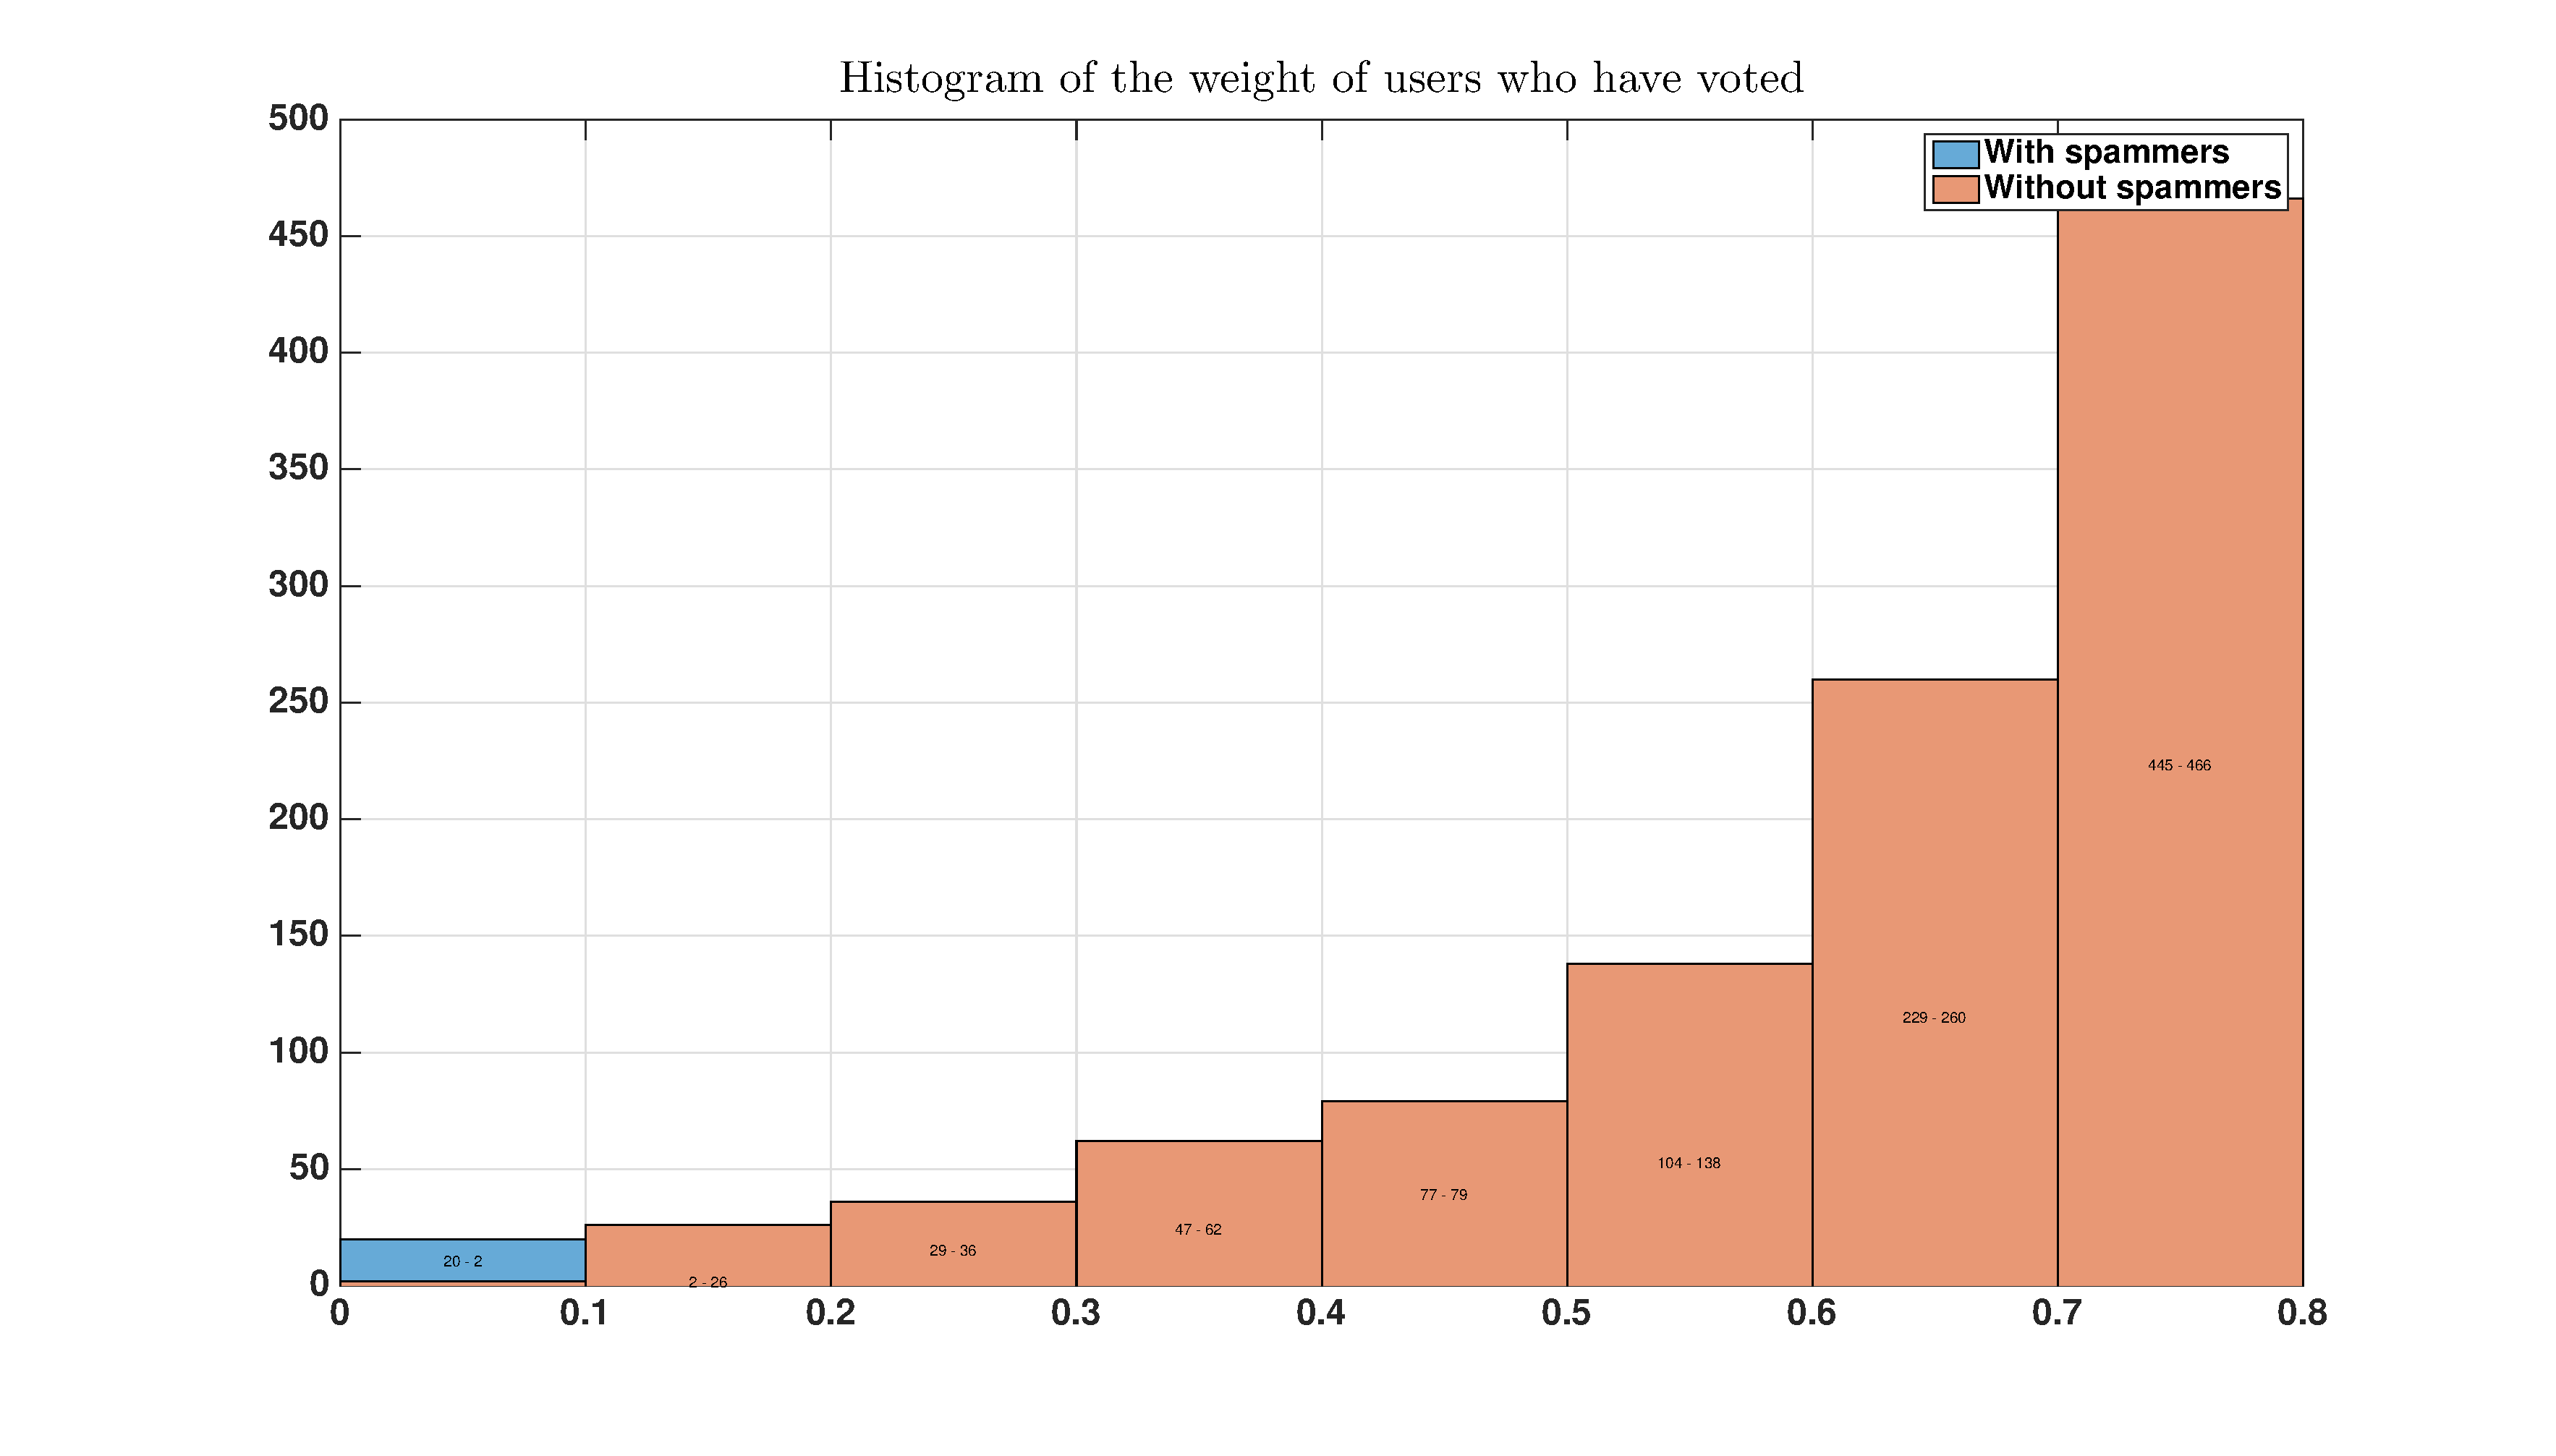
\includegraphics[width=\textwidth]{../rapport/images/hotels/not_random_cheaters.eps}
        \end{figure}
\end{frame}

\begin{frame}{Application \rom{2}: Hotels with spammers (2)}
    We now added to the original data set one spammer per hotel giving always 0 except for their own hotel, which they rated 5.
            \begin{figure}
            \centering
            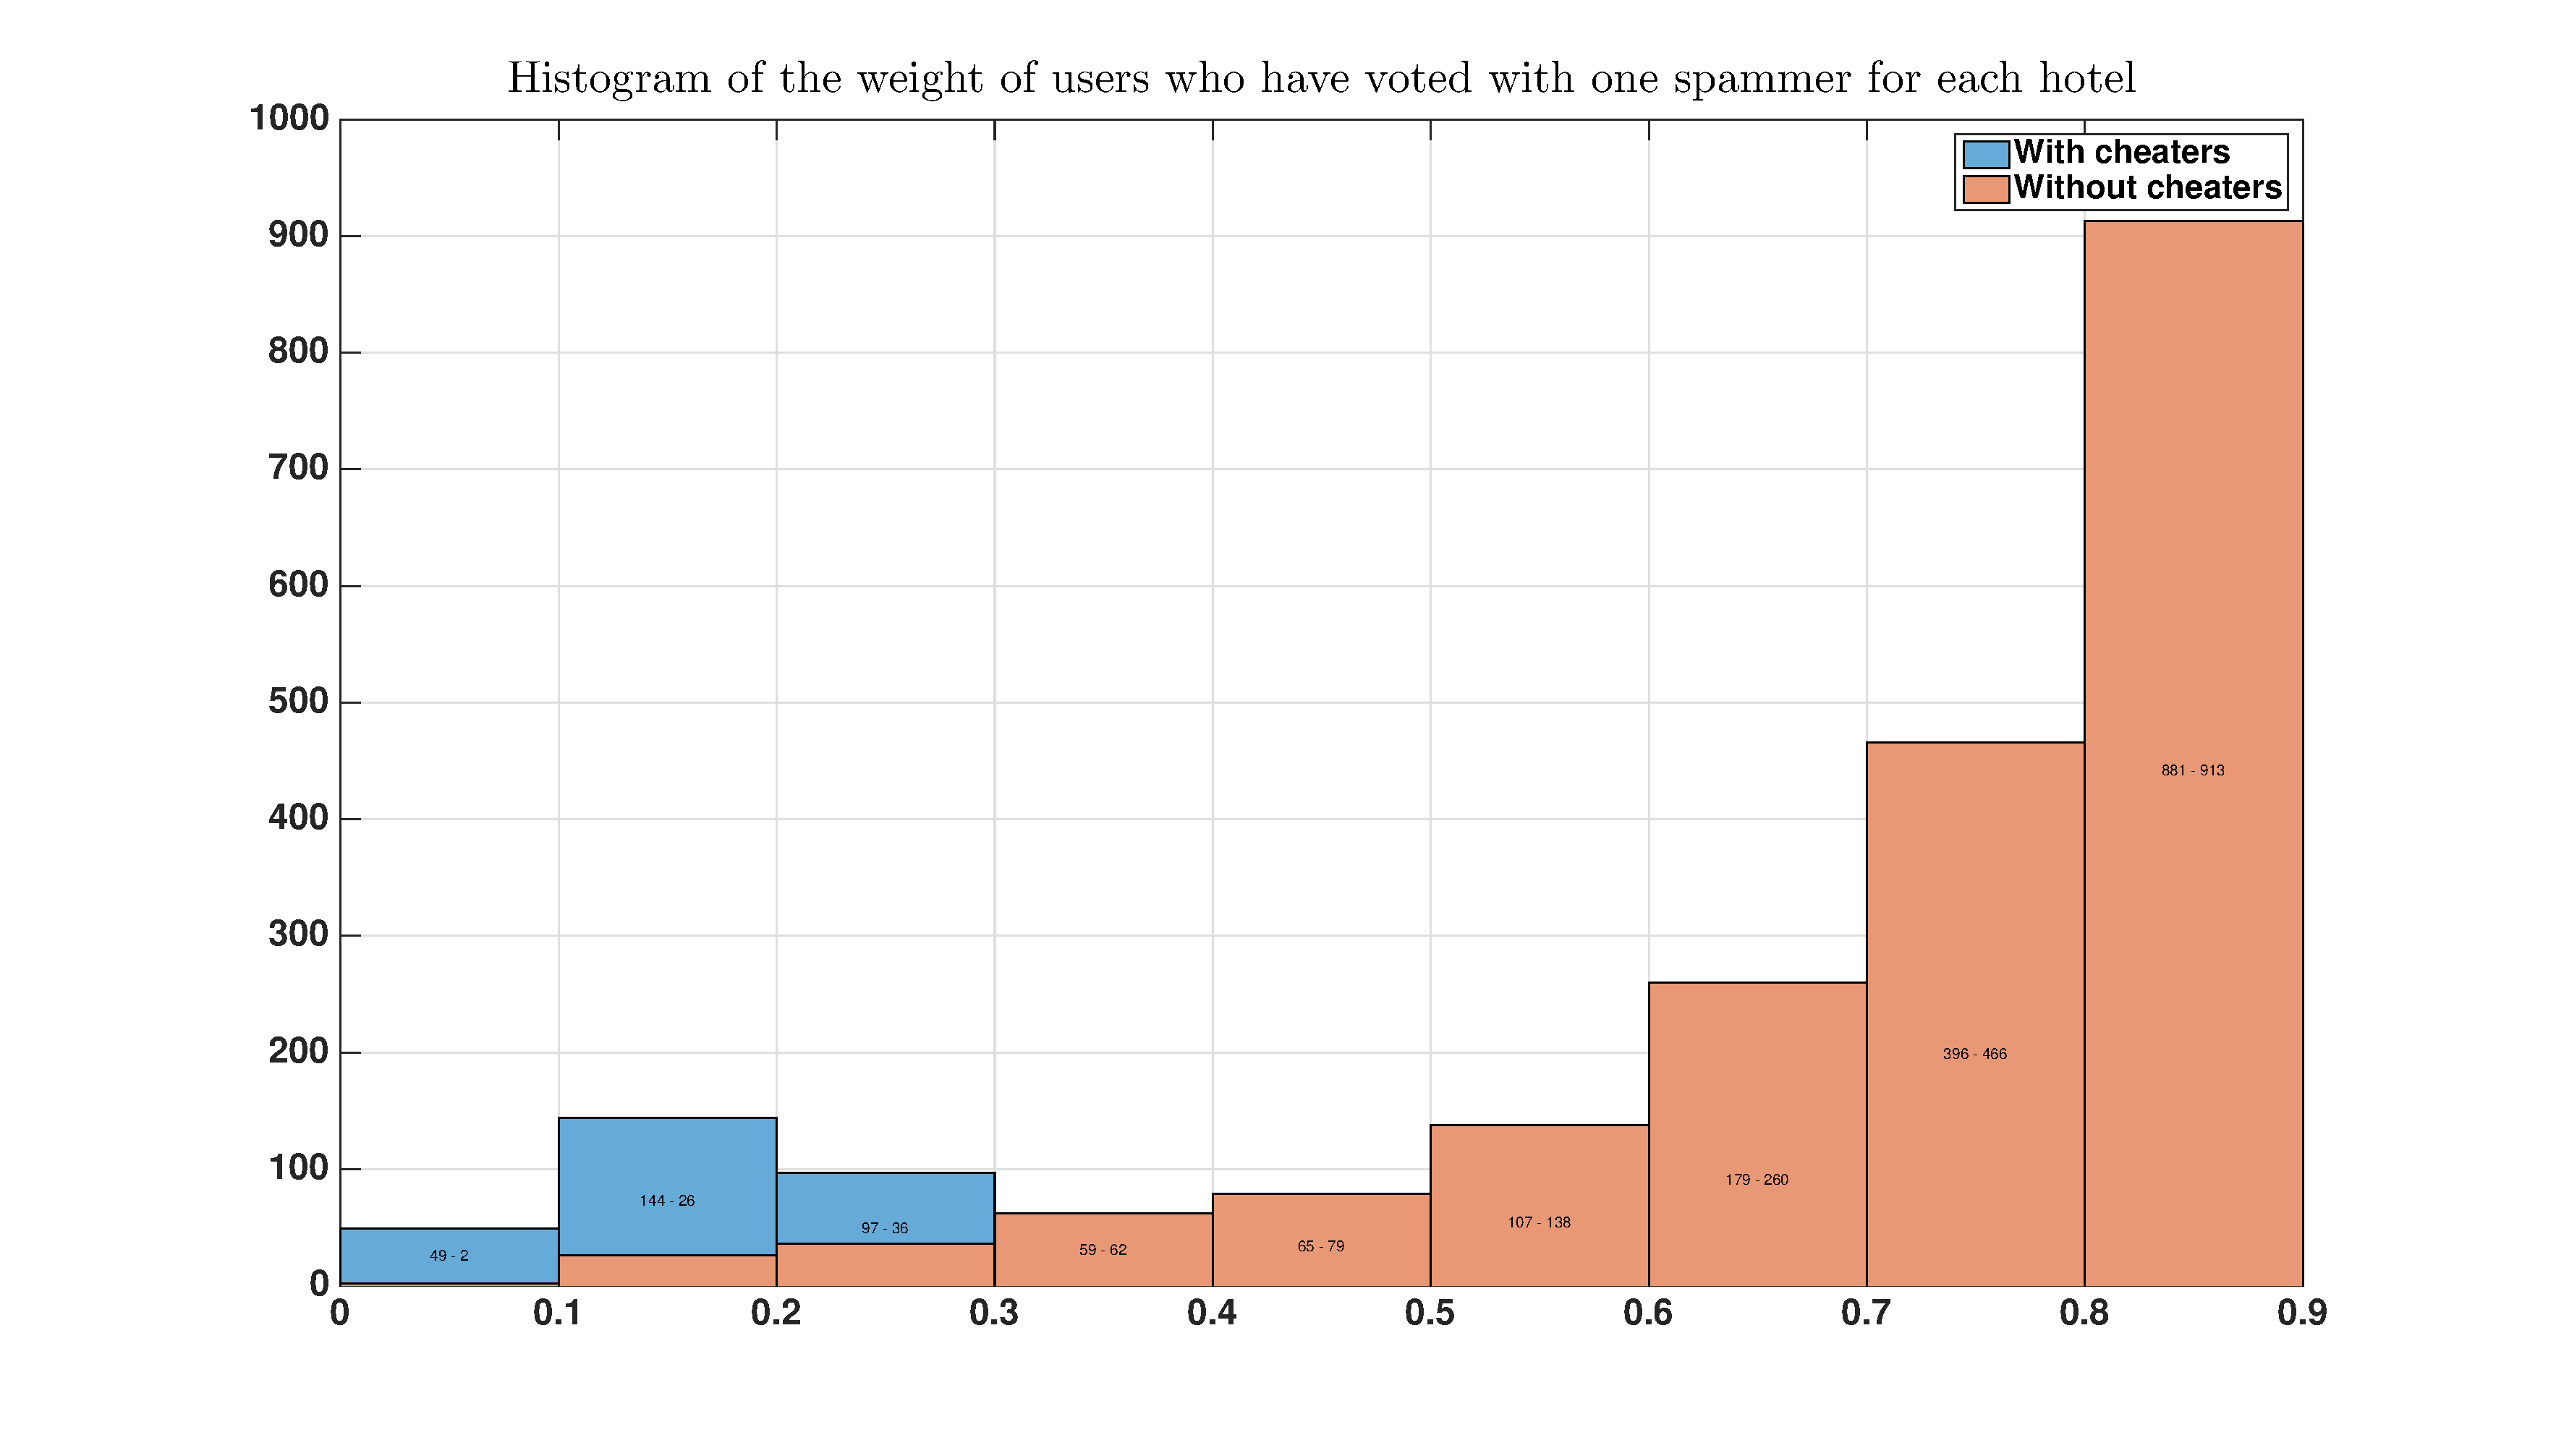
\includegraphics[width=\textwidth]{../rapport/images/hotels/not_random_each_hotels.eps}
        \end{figure}
\end{frame}

\begin{frame}{Conclusion}

\end{frame}